% !TeX program = xelatex
\documentclass[a4paper,10pt]{article}

% ============================================================================
% កញ្ចប់បណ្ណាល័យ (Packages) – តាមលំនាំ NGS Preah Krasang (ls_plan.tex)
% បរិបទ៖ គ្មានស្លាយ LCD និងគ្មានម៉ាស៊ីនគិតលេខ — ប្រើសន្លឹកកិច្ចការសិស្ស (ស-ខ្មៅ) និងក្ដារខៀនជាគោល
% ============================================================================
\usepackage[a4paper, left=0.95cm, right=0.95cm, top=0.85cm, bottom=0.92cm, footskip=0.52cm]{geometry}
\usepackage{amsmath}
\usepackage{unicode-math}
\usepackage{fontspec}
\usepackage{array, longtable, multirow, colortbl}
\usepackage[table]{xcolor}
\usepackage{enumitem}
\usepackage{pifont}
\usepackage{fancyhdr}
\usepackage{tikz}
\usetikzlibrary{calc, arrows.meta, angles, quotes, decorations.markings, decorations.pathreplacing, patterns, babel}

\makeatletter
\let\@expl@@@mark@update@singlecol@structures@@\relax
\makeatother

\providecommand{\NGSFindFonts}{%
  \IfFileExists{C:/Windows/Fonts/cambria.ttc}{%
    \def\NGSSysPath{C:/Windows/Fonts/}%
    \def\NGSUserPath{C:/Users/KIT/AppData/Local/Microsoft/Windows/Fonts/}%
  }{%
    \IfFileExists{./fonts/KhmerOSsiemreap.ttf}{\def\NGSSysPath{./fonts/}\def\NGSUserPath{./fonts/}}{%
    \IfFileExists{../fonts/KhmerOSsiemreap.ttf}{\def\NGSSysPath{../fonts/}\def\NGSUserPath{../fonts/}}{%
    \IfFileExists{../../fonts/KhmerOSsiemreap.ttf}{\def\NGSSysPath{../../fonts/}\def\NGSUserPath{../../fonts/}}{%
    \IfFileExists{../../../fonts/KhmerOSsiemreap.ttf}{\def\NGSSysPath{../../../fonts/}\def\NGSUserPath{../../../fonts/}}{%
    \IfFileExists{../../../../fonts/KhmerOSsiemreap.ttf}{\def\NGSSysPath{../../../../fonts/}\def\NGSUserPath{../../../../fonts/}}{%
    \IfFileExists{../../../../../fonts/KhmerOSsiemreap.ttf}{\def\NGSSysPath{../../../../../fonts/}\def\NGSUserPath{../../../../../fonts/}}{%
    \IfFileExists{../../../../../../fonts/KhmerOSsiemreap.ttf}{\def\NGSSysPath{../../../../../../fonts/}\def\NGSUserPath{../../../../../../fonts/}}{%
      \def\NGSSysPath{../../../../../../../fonts/}\def\NGSUserPath{../../../../../../../fonts/}%
    }}}}}}}%
  }%
}
\NGSFindFonts

\setmathfont[Path={\NGSSysPath}, FontIndex=1, Scale=1.02]{cambria.ttc}
\defaultfontfeatures{Ligatures=TeX}

\setmainfont[
  Path={\NGSUserPath}, Extension=.ttf, Script=Khmer,
  BoldFont={KhmerOSsiemreap}, BoldFeatures={FakeBold=1.8},
  ItalicFont={KhmerOSsiemreap}, ItalicFeatures={FakeSlant=0.25},
  BoldItalicFont={KhmerOSsiemreap}, BoldItalicFeatures={FakeBold=1.8, FakeSlant=0.25}
]{KhmerOSsiemreap}

\newfontfamily\muol[Path={\NGSUserPath}, Extension=.ttf, Script=Khmer]{KhmerOSmuollight}
\newfontfamily\TimesEn[Path={\NGSSysPath}, Extension=.ttf, Scale=1.00, BoldFont={timesbd}, ItalicFont={timesi}, BoldItalicFont={timesbi}]{times}
\newfontfamily\NagaBold[Path={\NGSUserPath}, Extension=.ttf]{AKbalthom Naga Bold}
\newfontfamily\CalibriFont[Path={\NGSSysPath}, Extension=.ttf]{calibri}
\newfontfamily\Tacteing[Path={\NGSUserPath}]{TACTENG.TTF}
\newfontfamily\CourierBullet[Path={\NGSSysPath}, Extension=.ttf]{cour}
\newcommand{\wcirc}{{\CourierBullet\fontsize{9.5pt}{11pt}\selectfont o}}

\XeTeXlinebreaklocale "km"
\XeTeXlinebreakskip = 0pt plus 1pt minus 0.1pt

\definecolor{stepgray}{HTML}{D9D9D9}
\definecolor{headgray}{HTML}{F2F2F2}
\definecolor{boxgray}{HTML}{D9D9D9}
\definecolor{darkred}{HTML}{C00000}
\definecolor{red5e}{HTML}{FF0000}

\pagestyle{fancy}
\fancyhf{}
\renewcommand{\headrulewidth}{0pt}
\fancyfoot[R]{\CalibriFont\fontsize{11pt}{13pt}\selectfont\thepage}

\setlength{\parindent}{0pt}
\setlength{\parskip}{0pt}
\setlength{\tabcolsep}{3.8pt}

\newcolumntype{L}[1]{>{\raggedright\arraybackslash}p{#1}}
\newcolumntype{C}[1]{>{\centering\arraybackslash}p{#1}}

\newcommand{\en}[1]{{\TimesEn #1}}
\newcommand{\enbf}[1]{{\TimesEn\textbf{#1}}}
\newcommand{\unit}[1]{\,\text{\en{#1}}}
\newcommand{\fiveE}[1]{{\NagaBold\fontsize{9.5pt}{13pt}\selectfont\textcolor{red5e}{#1}}}
\newcommand{\timenote}[1]{\textcolor{darkred}{\textit{#1}}}
\newcommand{\redsub}[1]{\textcolor{darkred}{#1}}
\newcommand{\graybox}[1]{\colorbox{boxgray}{\strut\hspace{2pt}#1\hspace{2pt}}}
\newcommand{\ditem}{\tikz[baseline=-0.5ex]\fill (0,0.42ex) -- (0.42ex,0) -- (0,-0.42ex) -- (-0.42ex,0) -- cycle;\hspace{0.3em}}
\newcommand{\cnum}[1]{{\fontsize{10.5pt}{12pt}\selectfont\ding{\numexpr181+#1\relax}}\hspace{0.15em}}
\newcommand{\cfig}[1]{\par\vspace{3pt}{\centering #1\par}\vspace{3pt}}
\newcommand{\stepheader}[1]{\multicolumn{3}{|c|}{\cellcolor{stepgray}\muol #1} \\* \noalign{\hrule height 0.4pt}}
\newcommand{\khmflourish}{{\Tacteing\fontsize{36pt}{14pt}\selectfont\raisebox{-5pt}{3}}}

% ============================================================================
% ម៉ាក្រូគូសរូប TikZ ស-ខ្មៅ ១០០% សម្រាប់មេរៀន ៣.១.៣ ទំហំសមាមាត្រច្រាស (INVP)
% ============================================================================

% ១. E1 Engage: អន្ទាក់គុណខ្វែងលើចំណោទកម្មករ 35 -> 28 នាក់ (ទំ.៣០-៣១)
\newcommand{\figEngageINVP}{%
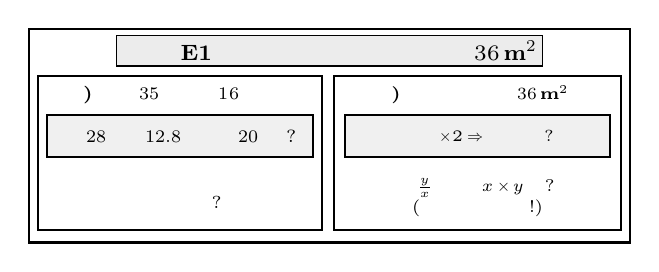
\begin{tikzpicture}[x=0.96cm, y=0.92cm, every node/.style={font=\scriptsize, text=black}]
  \draw[black, line width=0.95pt] (0,0) rectangle (7.95,2.95);
  \node[fill=gray!15, draw=black, line width=0.6pt, inner sep=2pt, font=\footnotesize\bfseries] at (3.975,2.65) {បេសកកម្ម \en{E1}៖ អន្ទាក់ការដ្ឋានសង់ផ្ទះ និងក្រឡាផ្ទៃថេរ $36\unit{m}^2$};

  \draw[black, line width=0.8pt] (0.12,0.18) rectangle (3.88,2.30);
  \node[font=\fontsize{6.4pt}{8.5pt}\selectfont\bfseries] at (2.00,2.04) {១) កម្មករ $35$ នាក់ សង់ $16$ ថ្ងៃចប់};
  \draw[black, line width=0.75pt, fill=gray!12] (0.24,1.18) rectangle (3.76,1.76);
  \node[font=\fontsize{6.4pt}{8pt}\selectfont] at (2.00,1.47) {ចុះ $28$ នាក់៖ $12.8$ ថ្ងៃ \;ឬ\; $20$ ថ្ងៃ?};
  \node[align=center, font=\fontsize{6.3pt}{7.8pt}\selectfont] at (2.00,0.62) {កម្មករ\textbf{ថយចុះ} តើចំនួនថ្ងៃត្រូវ\\\textbf{ថយចុះ} ឬ \textbf{កើនឡើង}?};

  \draw[black, line width=0.8pt] (4.04,0.18) rectangle (7.83,2.30);
  \node[font=\fontsize{6.2pt}{8pt}\selectfont\bfseries] at (5.935,2.04) {២) ចតុកោណកែងក្រឡាផ្ទៃថេរ $36\unit{m}^2$};
  \draw[black, line width=0.75pt, fill=gray!12] (4.18,1.18) rectangle (7.69,1.76);
  \node[font=\fontsize{5.8pt}{7.5pt}\selectfont] at (5.935,1.47) {ទទឹងកើន $\times 2 \Rightarrow$ បណ្ដោយយ៉ាងណា?};
  \node[align=center, font=\fontsize{6.1pt}{7.6pt}\selectfont] at (5.935,0.62) {តើ $\frac{y}{x}$ ថេរ \;ឬ\; $x\times y$ ថេរ?\\(ប្រៀបធៀបនឹងសមាមាត្រស្រប!)};
\end{tikzpicture}}

% ២. E2 POE 1: គ្រួសារចតុកោណកែងក្រឡាផ្ទៃថេរ S = 36 m^2 (ទំ.៣០)
\newcommand{\figAreaINVP}{%
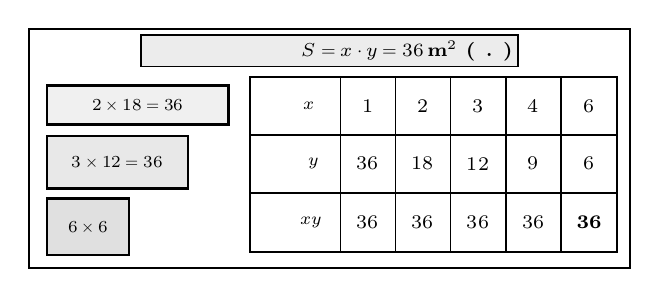
\begin{tikzpicture}[x=0.96cm, y=0.92cm, every node/.style={font=\scriptsize, text=black}]
  \draw[black, line width=0.95pt] (0,0) rectangle (7.95,3.30);
  \node[fill=gray!15, draw=black, line width=0.6pt, inner sep=2pt, font=\fontsize{6.8pt}{8.5pt}\selectfont\bfseries] at (3.975,3.00) {ពិសោធន៍ចតុកោណកែងក្រឡាផ្ទៃថេរ $S = x\cdot y = 36\unit{m}^2$ (ទំ.៣០)};

  % Rect 1: 2 x 18 (scaled)
  \draw[black, line width=0.85pt, fill=gray!12] (0.24,1.98) rectangle (2.64,2.52);
  \node[font=\fontsize{6.1pt}{7.6pt}\selectfont] at (1.44,2.25) {$2 \times 18 = 36$};

  % Rect 2: 3 x 12
  \draw[black, line width=0.85pt, fill=gray!18] (0.24,1.10) rectangle (2.10,1.82);
  \node[font=\fontsize{6.1pt}{7.6pt}\selectfont] at (1.17,1.46) {$3 \times 12 = 36$};

  % Rect 3: 6 x 6
  \draw[black, line width=0.85pt, fill=gray!24] (0.24,0.18) rectangle (1.32,0.96);
  \node[font=\fontsize{6.1pt}{7.6pt}\selectfont] at (0.78,0.57) {$6\times 6$};

  % Table on right
  \draw[black, line width=0.8pt] (2.92,0.22) rectangle (7.78,2.64);
  \draw[black, line width=0.6pt] (2.92,1.84) -- (7.78,1.84);
  \draw[black, line width=0.6pt] (2.92,1.04) -- (7.78,1.04);
  \draw[black, line width=0.6pt] (4.12,0.22) -- (4.12,2.64);
  \foreach \xx in {4.85, 5.58, 6.31, 7.04} {\draw[black, line width=0.5pt] (\xx,0.22) -- (\xx,2.64);}

  \node[font=\fontsize{6.2pt}{7.8pt}\selectfont] at (3.52,2.24) {\textbf{ទទឹង $x$}};
  \node[font=\fontsize{6.2pt}{7.8pt}\selectfont] at (3.52,1.44) {\textbf{បណ្ដោយ $y$}};
  \node[font=\fontsize{6.2pt}{7.8pt}\selectfont] at (3.52,0.63) {\textbf{ផលគុណ $xy$}};

  \node at (4.48,2.24) {$1$};  \node at (5.21,2.24) {$2$};  \node at (5.94,2.24) {$3$};  \node at (6.67,2.24) {$4$};  \node at (7.41,2.24) {$6$};
  \node at (4.48,1.44) {$36$}; \node at (5.21,1.44) {$18$}; \node at (5.94,1.44) {$12$}; \node at (6.67,1.44) {$9$};  \node at (7.41,1.44) {$6$};
  \node at (4.48,0.63) {$36$}; \node at (5.21,0.63) {$36$}; \node at (5.94,0.63) {$36$}; \node at (6.67,0.63) {$36$}; \node at (7.41,0.63) {$\mathbf{36}$};
\end{tikzpicture}}

% ៣. E4 Worked Example: កម្មករ 35 នាក់ x 16 ថ្ងៃ = 28 នាក់ x x ថ្ងៃ (ទំ.៣០-៣១)
\newcommand{\figWorkersINVP}{%
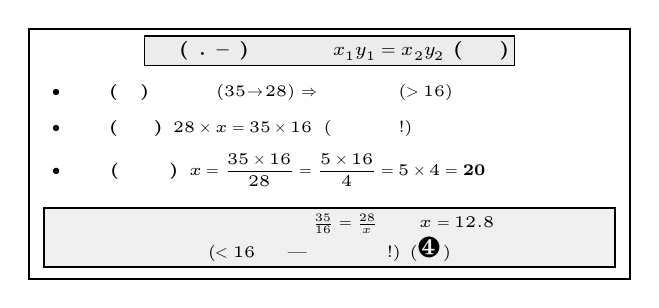
\begin{tikzpicture}[x=0.96cm, y=0.92cm, every node/.style={font=\scriptsize, text=black}]
  \draw[black, line width=0.95pt] (0,0) rectangle (7.95,3.45);
  \node[fill=gray!15, draw=black, line width=0.6pt, inner sep=2pt, font=\fontsize{6.8pt}{8.5pt}\selectfont\bfseries] at (3.975,3.15) {គំរូ (ទំ.៣០–៣១)៖ ច្រកផលគុណថេរ $x_1 y_1 = x_2 y_2$ (សង់ផ្ទះ)};

  \node[anchor=west, font=\fontsize{5.8pt}{7.5pt}\selectfont] at (0.18,2.58) {$\bullet$ \textbf{ជំហាន ១ (ទិសដៅ)៖} កម្មករថយចុះ ($35\!\to\! 28$) $\Rightarrow$ ចំនួនថ្ងៃកើនឡើង ($>16$)};
  \node[anchor=west, font=\fontsize{5.8pt}{7.5pt}\selectfont] at (0.18,2.08) {$\bullet$ \textbf{ជំហាន ២ (ផលគុណថេរ)៖} $28 \times x = 35 \times 16$ \;(ហាមគុណខ្វែងស្រប!)};
  \node[anchor=west, font=\fontsize{5.9pt}{7.6pt}\selectfont] at (0.18,1.50) {$\bullet$ \textbf{ជំហាន ៣ (សម្រួលដោយដៃ)៖} $x = \dfrac{35\times 16}{28} = \dfrac{5\times 16}{4} = 5\times 4 = \mathbf{20\text{ ថ្ងៃ}}$};

  \draw[black, line width=0.75pt, fill=gray!12] (0.20,0.16) rectangle (7.75,0.98);
  \node[align=center, font=\fontsize{5.9pt}{7.5pt}\selectfont] at (3.975,0.57) {\textbf{ប្រយ័ត្នអន្ទាក់គុណខ្វែងស្រប៖} បើសរសេរ $\frac{35}{16}=\frac{28}{x}$ នឹងបាន $x=12.8$ ថ្ងៃ\\($<16$ ថ្ងៃ — ខុសទំនងហេតុផលពិត!) (\cnum{4})};
\end{tikzpicture}}

% ៤. E5 Diagnostic Options A-D
\newcommand{\figExitCardsINVP}{%
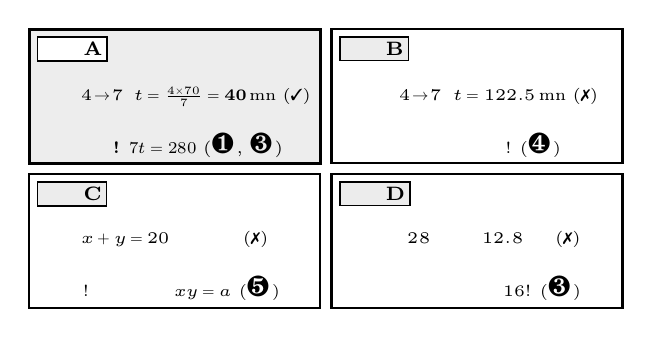
\begin{tikzpicture}[x=0.96cm, y=0.92cm, every node/.style={font=\scriptsize, text=black}]
  \draw[black, line width=1.1pt, fill=gray!14] (0,2.00) rectangle (3.85,3.85);
  \node[anchor=north west, fill=white, draw=black, line width=0.6pt, inner sep=1.8pt] at (0.10,3.75) {\textbf{ជម្រើស \en{A}}};
  \node[font=\fontsize{5.8pt}{7.5pt}\selectfont] at (1.925,2.92) {រ៉ូប៊ីណេ $4\!\to\! 7$៖ $t=\frac{4\times 70}{7}=\mathbf{40\unit{mn}}$ (\ding{51})};
  \node[font=\fontsize{6.0pt}{7.8pt}\selectfont] at (1.925,2.25) {\textbf{ត្រឹមត្រូវ!} $7t = 280$ (\cnum{1}, \cnum{3})};

  \draw[black, line width=0.9pt] (4.00,2.00) rectangle (7.85,3.85);
  \node[anchor=north west, fill=gray!15, draw=black, line width=0.6pt, inner sep=1.8pt] at (4.10,3.75) {\textbf{ជម្រើស \en{B}}};
  \node[font=\fontsize{5.9pt}{7.6pt}\selectfont] at (5.925,2.92) {រ៉ូប៊ីណេ $4\!\to\! 7$៖ $t = 122.5\unit{mn}$ (\ding{55})};
  \node[font=\fontsize{5.8pt}{7.5pt}\selectfont] at (5.925,2.25) {ច្រឡំគុណខ្វែងសមាមាត្រស្រប! (\cnum{4})};

  \draw[black, line width=0.9pt] (0,0) rectangle (3.85,1.85);
  \node[anchor=north west, fill=gray!15, draw=black, line width=0.6pt, inner sep=1.8pt] at (0.10,1.75) {\textbf{ជម្រើស \en{C}}};
  \node[font=\fontsize{5.9pt}{7.6pt}\selectfont] at (1.925,0.95) {$x + y = 20$ សមាមាត្រច្រាស (\ding{55})};
  \node[font=\fontsize{5.8pt}{7.5pt}\selectfont] at (1.925,0.28) {ខុស! ផលបូកថេរ មិនមែន $xy=a$ (\cnum{5})};

  \draw[black, line width=0.9pt] (4.00,0) rectangle (7.85,1.85);
  \node[anchor=north west, fill=gray!15, draw=black, line width=0.6pt, inner sep=1.8pt] at (4.10,1.75) {\textbf{ជម្រើស \en{D}}};
  \node[font=\fontsize{5.9pt}{7.6pt}\selectfont] at (5.925,0.95) {កម្មករ $28$ នាក់ សង់ $12.8$ ថ្ងៃ (\ding{55})};
  \node[font=\fontsize{5.8pt}{7.5pt}\selectfont] at (5.925,0.28) {កម្មករតិច ថ្ងៃត្រូវច្រើនជាង $16$! (\cnum{3})};
\end{tikzpicture}}

\begin{document}
\fontsize{10pt}{15.2pt}\selectfont

% -------------------- ក្បាលកិច្ចតែងការ --------------------
\begin{center}
  {\muol\fontsize{11pt}{16pt}\selectfont ព្រះរាជាណាចក្រកម្ពុជា}\\[2pt]
  {\muol\fontsize{10pt}{15pt}\selectfont ជាតិ សាសនា ព្រះមហាក្សត្រ}\\[1pt]
  \khmflourish
\end{center}

\vspace{-24pt}
{\muol\fontsize{9.5pt}{12.5pt}\selectfont
មន្ទីរអប់រំ យុវជន និងកីឡា ខេត្តកំពង់ធំ\\
ការិយាល័យអប់រំ យុវជន និងកីឡា ស្រុកកំពង់ស្វាយ\\
អនុវិទ្យាល័យព្រះក្រសាំង}

\vspace{1pt}
\begin{center}
  {\muol\fontsize{10pt}{14pt}\selectfont កិច្ចតែងការបង្រៀន}
\end{center}
\vspace{0pt}

% -------------------- ព័ត៌មានទូទៅ --------------------
{\renewcommand{\arraystretch}{0.98}
\hspace*{3.1cm}%
\begin{tabular}{@{}l l L{11.0cm}@{}}
  - \hspace{0.35cm} មុខវិជ្ជា & : & គណិតវិទ្យា ថ្នាក់ទី៨ (ពីជគណិត) \\
  - \hspace{0.35cm} ចំណងជើងមេរៀន & : & មេរៀនទី៣៖ ទំហំសមាមាត្រ និងភាគរយ \\
  - \hspace{0.35cm} ចំណងជើងរង & : & ១.៣. ទំហំសមាមាត្រច្រាស (សៀវភៅពុម្ព ទំ.៣០–៣១ និងលំហាត់ \#6ឃ-ង, \#8, \#9, \#13 ទំ.៤០–៤១) \\
  - \hspace{0.35cm} រយៈពេល & : & ១ ម៉ោងសិក្សា (៥០ នាទី) \\
  - \hspace{0.35cm} បង្រៀនដោយ & : & ហុក ប៊ុនថែន \\
  - \hspace{0.35cm} កាលបរិច្ឆេទ & : & ថ្ងៃសុក្រ ទី២៧ ខែវិច្ឆិកា ឆ្នាំ២០២៦ \\
\end{tabular}

\vspace{2pt}

% -------------------- I. វត្ថុបំណង --------------------
\textbf{I.} {\muol វត្ថុបំណង}\\[1pt]
\hspace*{0.55cm}%
\begin{tabular}{@{}l l L{14.2cm}@{}}
  \wcirc \hspace{0.25cm} វិជ្ជាសម្បទា & : & សិស្សប្រាប់និយមន័យទំហំសមាមាត្រច្រាសតាមរយៈផលគុណថេរ $xy = a$ (ឬ $y = \dfrac{a}{x}$ ដែល $a\neq 0$) និងបែងចែកដាច់រវាងសមាមាត្រស្រប ($\frac{y}{x}=a$) នឹងសមាមាត្រច្រាស ($xy=a$) ។ \\
  \wcirc \hspace{0.25cm} បំណិនសម្បទា & : & សិស្សពិនិត្យតារាងតម្លៃ សរសេរសមីការ $y=\dfrac{a}{x}$ និងដោះស្រាយចំណោទជីវភាពសមាមាត្រច្រាស (កម្មករសង់ផ្ទះ និងក្បាលរ៉ូប៊ីណេបង្ហូរទឹក ទំ.៣០–៣១, ៤១) ដោយមិនច្រឡំគុណខ្វែងស្រប ។ \\
  \wcirc \hspace{0.25cm} ចរិយាសម្បទា & : & សិស្សមានទម្លាប់ពិនិត្យទំនងហេតុផលនៃទិសដៅកើន-ថយមុនគណនា និងឱ្យតម្លៃលើការរៀបចំកម្លាំងពលកម្មក្នុងជីវភាពរស់នៅ ។ \\
\end{tabular}

\vspace{2pt}

% -------------------- II. សម្ភារៈឧបទេស --------------------
\textbf{II.} {\muol សម្ភារៈឧបទេស}\\[1pt]
\hspace*{0.55cm}$\bullet$ \hspace{0.35cm} សៀវភៅសិក្សាគោលគណិតវិទ្យាថ្នាក់ទី៨ (ទំ.៣០–៣១, ៤០–៤១) ក្ដារខៀន ដីស និងសន្លឹកកិច្ចការសិស្ស ស-ខ្មៅ (\en{Worksheet\_INVP} ទំព័រ ១–២ គ្មានស្លាយ \en{LCD})

\vspace{2pt}

% -------------------- III. វិធីសាស្រ្តបង្រៀន --------------------
\textbf{III.} {\muol វិធីសាស្រ្តបង្រៀន}\\[1pt]
\hspace*{0.45cm}%
\begin{tabular}{@{}l l L{14.85cm}@{}}
  $\bullet$ \hspace{0.25cm} គោលវិធី & : & សិស្សមជ្ឈមណ្ឌល (បង្រៀនតាមសន្លឹកកិច្ចការស៊ើបអង្កេត និងក្ដារខៀន គ្មាន \en{LCD}) \\
  $\bullet$ \hspace{0.25cm} យុទ្ធវិធីបង្រៀន & : & គំរូ \en{5Es} រួមបញ្ចូលច្រកត្រួតពិនិត្យផលគុណថេរ $x_1 y_1 = x_2 y_2 = a$ ប្រឆាំងអន្ទាក់គុណខ្វែងសមាមាត្រស្រប (\en{Anti-Overuse of Cross-Multiplication}) \\
\end{tabular}
}

\vspace{2pt}

% -------------------- IV. ដំណើរការបង្រៀន --------------------
\textbf{IV.} {\muol ដំណើរការបង្រៀន}

\vspace{1pt}

\renewcommand{\arraystretch}{1.15}
\begin{longtable}{|L{5.50cm}|L{7.90cm}|L{4.80cm}|}
\hline
\rowcolor{headgray}
\multicolumn{1}{|c|}{\muol សកម្មភាពគ្រូ} &
\multicolumn{1}{c|}{\muol ខ្លឹមសារមេរៀន} &
\multicolumn{1}{c|}{\muol សកម្មភាពសិស្ស} \\
\hline
\endfirsthead
\hline
\endhead
\hline
\endfoot
\hline
\endlastfoot

% ==================== ជំហានទី១ (2min) ====================
\stepheader{ជំហានទី១ \enbf{(}រដ្ឋបាលថ្នាក់\enbf{)}}
$\bullet$ ពិនិត្យអវត្តមាន អនាម័យ និងសណ្ដាប់ធ្នាប់ថ្នាក់រៀន
&
$\bullet$ រដ្ឋបាលថ្នាក់ និងការរៀបចំដៃគូសិក្សា
&
$\circ$ ប្រធានថ្នាក់រាយការណ៍អវត្តមាន \\[3pt]

$\bullet$ ចែក \textbf{សន្លឹកកិច្ចការសិស្ស (\en{Worksheet\_INVP})} ម្នាក់ ១ សន្លឹក (ផ្កាប់ទុកសិន)
&
$\bullet$ សន្លឹកកិច្ចការសិស្ស ស-ខ្មៅ (\en{Worksheet\_INVP} ទំព័រ ១–២)
&
$\circ$ ទទួលសន្លឹកកិច្ចការ និងត្រៀមសម្ភារៈសរសេរ \\
\hline

% ==================== ជំហានទី២ (9min: <=3 + 3 + E1 3) ====================
\stepheader{ជំហានទី២ \enbf{(}កិច្ចការផ្ទះ \enbf{+} ទំនាក់ទំនងមេរៀនថ្មី\enbf{)}}
\ditem \textbf{កំណែកិច្ចការផ្ទះ ($\le 3\unit{min}$)} \timenote{(កុំសរសេរវែង)} \par
$\bullet$ ហៅសិស្ស ២ នាក់ឡើងសរសេរចម្លើយលំហាត់ \#5ក, \#11 និង \#12 (ទំ.៤០–៤១) លើក្ដារខៀន
&
{\centering\redsub{កំណែកិច្ចការផ្ទះមេរៀន ១.២ (ទំ.៤០–៤១ \#5ក, \#11, \#12)}\par} \par
$\bullet$ \textbf{\#5ក៖} អនុវត្តផលគុណតួចុងស្មើផលគុណតួមធ្យម \par
$\bullet$ \textbf{\#11 និង \#12៖} បែងចែកសមាមាត្រតាមផលបូកចំណែកសរុប
&
$\circ$ ផ្ទៀងផ្ទាត់ចម្លើយក្នុងសៀវភៅកិច្ចការផ្ទះ \\[3pt]

\ditem \textbf{រំលឹកមេរៀនទាក់ទង (3min)} \par
$\bullet$ សួររហ័ស៖ រំលឹករូបមន្តក្រឡាផ្ទៃចតុកោណកែង $S = x\times y$ និងរកគូចំនួនគត់វិជ្ជមានដែលគុណគ្នាបាន $36$
&
{\centering\redsub{រំលឹកក្រឡាផ្ទៃចតុកោណកែង និងគូកត្តានៃ $36$}\par} \par
$\bullet$ $1\times 36 = 2\times 18 = 3\times 12 = 4\times 9 = 6\times 6 = \mathbf{36}$
&
$\circ$ ឆ្លើយរហ័សរកគូកត្តាទាំង ៥ គូដែលមានផលគុណស្មើ $36$ \\[3pt]

\fiveE{E1 - Engage (3min)} \timenote{(កុំទាន់ផ្ដល់ចម្លើយ)} \par
\ditem \textbf{«បេសកកម្មការដ្ឋានសង់ផ្ទះ៖ អន្ទាក់គុណខ្វែង ១២.៨ ថ្ងៃ ទល់នឹង ២០ ថ្ងៃ!»} \par
$\bullet$ ឱ្យសិស្សបើកសន្លឹកកិច្ចការទំព័រ ១ គូសធីកទស្សន៍ទាយលើសំណួរ ២
&
{\centering\redsub{បេសកកម្ម E1៖ កម្មករសង់ផ្ទះ (ទំ.៣០) និងក្រឡាផ្ទៃថេរ $36\unit{m}^2$}\par} \par
$\bullet$ \textbf{សំណួរ ១៖} កម្មករ $35$ នាក់សង់ផ្ទះចប់ក្នុង $16$ ថ្ងៃ — បើនៅសល់កម្មករ $28$ នាក់ តើត្រូវប្រើពេល $12.8$ ថ្ងៃ ឬ $20$ ថ្ងៃ? \par
$\bullet$ \textbf{សំណួរ ២៖} ចតុកោណកែងក្រឡាផ្ទៃថេរ $36\unit{m}^2$ — តើ $\frac{y}{x}$ ថេរ ឬ $x\times y$ ថេរ?
&
$\circ$ គូសធីកទស្សន៍ទាយលើសន្លឹកកិច្ចការទំព័រ ១ \\[3pt]

&
\cfig{\figEngageINVP}
& \\[3pt]

$\bullet$ ស្រង់ចំនួនដៃសិស្សកត់លើក្ដារខៀន (មិនទាន់ប្រាប់ចម្លើយត្រូវ)
&
$\bullet$ ស្ថិតិទស្សន៍ទាយ៖ $12.8$ ថ្ងៃ ទល់នឹង $20$ ថ្ងៃ ; $\frac{y}{x}$ ថេរ ទល់នឹង $xy$ ថេរ
&
$\circ$ លើកដៃបង្ហាញការទស្សន៍ទាយ \\
\hline

% ==================== ជំហានទី៣ (17min: E2 11m + E3 6m) ====================
\stepheader{ជំហានទី៣ \enbf{(}ខ្លឹមសារមេរៀនថ្មី\enbf{)}}
\fiveE{E2 - Explore (11min)} \par
$\bullet$ សរសេរចំណងជើងរងលើក្ដារខៀន
&
\textbf{១.៣. ទំហំសមាមាត្រច្រាស} (សៀវភៅពុម្ព ទំ.៣០–៣១)
&
$\circ$ កត់ចំណងជើងចូលសៀវភៅ \\[3pt]

\ditem \textbf{សកម្មភាព ១៖ តារាងចតុកោណកែងក្រឡាផ្ទៃថេរ $36\unit{m}^2$ \en{POE 1} (6min, ទំ.៣០)} \par
$\bullet$ ឱ្យដៃគូបំពេញតារាងទទឹង $x$ បណ្ដោយ $y$ និងផលគុណ $x\cdot y$ លើសន្លឹកកិច្ចការ
&
{\centering\textbf{សកម្មភាព ១ (\en{POE 1})៖ ចតុកោណកែងក្រឡាផ្ទៃថេរ $S = 36\unit{m}^2$}\par} \par
$\bullet$ ពេល $x$ កើន $\times 2$ ($1\to 2$) នោះ $y$ ថយ $\div 2$ ($36\to 18$) \par
$\bullet$ គ្រប់ជួរឈរមានផលគុណថេរ៖ $x\cdot y = \mathbf{36} \implies y = \dfrac{36}{x}$ (សមាមាត្រច្រាស!)
&
$\circ$ បំពេញតារាង និងរកឃើញថាផលគុណ $xy = 36$ ថេរគ្រប់គូតម្លៃ \\[3pt]

&
\cfig{\figAreaINVP}
& \\[3pt]

\ditem \textbf{សកម្មភាព ២៖ ញែកដាច់ ស្រប ទល់នឹង ច្រាស ទល់នឹង អន្ទាក់ដកថេរ \en{POE 2} (5min)} \par
$\bullet$ ឱ្យដៃគូប្រៀបធៀបតារាង ៣ ប្រភេទ៖ $\frac{y}{x}=a$ (ស្រប), $xy=a$ (ច្រាស), និង $x+y=20$ (ផលបូកថេរ)
&
{\centering\textbf{សកម្មភាព ២ (\en{POE 2})៖ ប្រៀបធៀប ៣ ទំនាក់ទំនង}\par} \par
$\bullet$ \textbf{សមាមាត្រស្រប៖} $\frac{y}{x} = a$ ថេរ \;;\; \textbf{សមាមាត្រច្រាស៖} $x\cdot y = a$ ថេរ \par
$\bullet$ \textbf{អន្ទាក់ដកថេរ ($x+y=20$)៖} ទោះ $x$ កើន ហើយ $y$ ថយក៏ដោយ ក៏ $x\cdot y$ មិនថេរដែរ ($5\times 15=75 \neq 10\times 10=100$) — មិនមែនសមាមាត្រច្រាសទេ!
&
$\circ$ ពិនិត្យផលគុណ $xy$ និងបំបែកអន្ទាក់ «ឱ្យតែមួយកើនមួយថយ គឺច្រាស» \\[3pt]

% --- E3 Explain (6min) ---
\fiveE{E3 - Explain (6min)} \par
\ditem \textbf{បង្គុំនិយមន័យ «ជាទូទៅ» (ទំ.៣០) និងធនាគារហេតុផល (ផ្នែកទី២)} \par
$\bullet$ ឱ្យសិស្សបង្គុំប្រអប់ \textbf{ជាទូទៅ (ទំ.៣០)} និងទំនាក់ទំនងពីរគូតម្លៃ $x_1 y_1 = x_2 y_2$
&
$\bullet$ \textbf{ជាទូទៅ (ទំ.៣០)៖} ប្រសិនបើទំហំ $y$ សមាមាត្រច្រាសនឹងទំហំ $x$ គេបាន៖ \par
{\centering\graybox{$xy = a$ \;;\; $y = \dfrac{a}{x}$ \;($a \neq 0$)}\par} \par
ដែល $a$ ជាមេគុណសមាមាត្រ ហើយចំពោះពីរគូតម្លៃ៖ $\mathbf{x_1 y_1 = x_2 y_2} \iff \dfrac{x_1}{x_2} = \dfrac{y_2}{y_1}$ ។
&
$\circ$ បំពេញប្រអប់ «ជាទូទៅ» លើសន្លឹកកិច្ចការ និងកត់ចូលសៀវភៅ \\[3pt]

$\bullet$ សង្ខេប \textbf{ធនាគារហេតុផល \cnum{1}--\cnum{2}} អំពីផលគុណថេរ និងទិសដៅកើន-ថយ
&
\textbf{ធនាគារហេតុផល \en{B\&W} (\cnum{1}--\cnum{5})៖} \par
\cnum{1} និយមន័យសមាមាត្រច្រាស៖ ផលគុណ $x\cdot y = a$ ថេរជានិច្ច $\iff y = \frac{a}{x}$ ($a\neq 0$) \par
\cnum{2} លក្ខណៈពហុគុណច្រាស៖ បើ $x$ គុណនឹង $k$ នោះ $y$ ត្រូវចែកនឹង $k$
&
$\circ$ ផ្ទៀងផ្ទាត់ហេតុផល \cnum{1}--\cnum{2} លើសន្លឹកកិច្ចការ \\[3pt]

$\bullet$ សង្ខេប \textbf{ធនាគារហេតុផល \cnum{3}} អំពីច្បាប់ផលគុណស្មើគ្នា
&
\cnum{3} ច្បាប់ផលគុណស្មើគ្នា៖ $x_1 y_1 = x_2 y_2$ (បរិមាណការងារសរុបមិនប្រែប្រួល)
&
$\circ$ ផ្ទៀងផ្ទាត់ហេតុផល \cnum{3} លើសន្លឹកកិច្ចការ \\[3pt]

$\bullet$ សង្ខេប \textbf{ធនាគារហេតុផល \cnum{4}--\cnum{5}} សម្រាប់ការពារអន្ទាក់គុណខ្វែងស្រប និងអន្ទាក់ផលបូកថេរ
&
\cnum{4} ការពារអន្ទាក់គុណខ្វែងស្រប៖ ហាមសរសេរ $\frac{x_1}{y_1}=\frac{x_2}{y_2}$ លើចំណោទសមាមាត្រច្រាស! \par
\cnum{5} អន្ទាក់ផលបូកថេរ៖ $y = c - x$ ($x+y=c$) មិនមែនសមាមាត្រច្រាសទេ ព្រោះ $xy$ មិនថេរ
&
$\circ$ ផ្ទៀងផ្ទាត់ហេតុផល \cnum{4}--\cnum{5} លើសន្លឹកកិច្ចការ \\
\hline

% ==================== ជំហានទី៤ (20min: E4 10m + E5 10m) ====================
\stepheader{ជំហានទី៤ \enbf{(}ពង្រីកចំណេះដឹង និងវាយតម្លៃ\enbf{)}}
\fiveE{E4 - Elaborate (10min)} \par
\ditem \textbf{លំហាត់គំរូ៖ កម្មករសង់ផ្ទះ (ទំ.៣០–៣១ — សន្លឹកកិច្ចការ ទំព័រ ២ ផ្នែកទី៣)} \par
$\bullet$ ដឹកនាំដោះស្រាយ \textbf{គំរូកម្មករ $35$ នាក់សង់ $16$ ថ្ងៃ ចុះ $28$ នាក់សង់ប៉ុន្មានថ្ងៃ?} តាមច្រកទ្វារ ៣ ជំហាន
&
{\muol លំហាត់គំរូទី ១} \textbf{(ទំ.៣០–៣១ — កម្មករសង់ផ្ទះ)៖} \par
$\bullet$ ចំនួនកម្មករ និងចំនួនថ្ងៃជាទំហំ\textbf{សមាមាត្រច្រាស} ($28 < 35 \implies x > 16$ ថ្ងៃ) \par
$\bullet$ តាមផលគុណថេរ៖ $28\cdot x = 35\times 16 \implies x = \dfrac{35\times 16}{28} = \dfrac{5\times 16}{4} = \mathbf{20\text{ ថ្ងៃ}}$ (\cnum{3})
&
$\circ$ អនុវត្តច្រកទ្វារ ៣ ជំហាន និងសម្រួលប្រភាគដោយដៃលើសន្លឹកកិច្ចការ \\[3pt]

$\bullet$ ដឹកនាំ \textbf{លំហាត់គំរូទី ២ (ពិនិត្យតារាង \#6ឃ ទំ.៤០ និងសរសេរសមីការ \#8 ទំ.៤១)}
&
{\muol លំហាត់គំរូទី ២} \textbf{(ពិនិត្យតារាង និងរកមេគុណសមាមាត្រច្រាស)៖} \par
$\bullet$ បើ $y$ សមាមាត្រច្រាសនឹង $x$ ហើយពេល $x=6 \Rightarrow y=8$ នោះ $a = 6\times 8 = 48 \implies \mathbf{y = \dfrac{48}{x}}$ (\cnum{1})
&
$\circ$ គណនាមេគុណ $a = xy$ និងសរសេរសមីការ $y = \frac{a}{x}$ \\[3pt]

&
\cfig{\figWorkersINVP}
& \\[3pt]

$\bullet$ សួរសំណួរឆ្លុះបញ្ចាំង \textbf{\en{EIA Looking-Back} (៣០ វិនាទី)}
&
\textbf{\en{EIA Looking-Back}៖} «ពេលណាយើងប្រើ $\dfrac{y_1}{x_1}=\dfrac{y_2}{x_2}$ ហើយពេលណាយើងប្រើ $x_1 y_1 = x_2 y_2$?»
&
$\circ$ ឆ្លើយ៖ «បើមួយកើនមួយទៀតកើនតាមពហុគុណប្រើ $\frac{y}{x}=a$ ; បើមួយកើនមួយទៀតថយតាមពហុគុណប្រើ $xy=a$!» \\[3pt]

% --- E5 Evaluate (10min) ---
\fiveE{E5 - Evaluate (10min)} \par
\ditem \textbf{ហ្វឹកហាត់ជាដៃគូលើ «ប្រតិបត្តិ» (6min, ទំ.៣១ — ផ្នែកទី៤-ក)} \par
$\bullet$ ឱ្យដៃគូធ្វើ \textbf{ប្រតិបត្តិ (ទំ.៣១ លើ — ក្បាលរ៉ូប៊ីណេទឹក $4 \to 7$)}
&
{\muol លំហាត់ប្រតិបត្តិ} \textbf{(ទំ.៣១ លើ និងពង្រឹង \#9 ទំ.៤១)៖} \par
$\bullet$ \textbf{១) ប្រតិបត្តិ (ទំ.៣១)៖} រ៉ូប៊ីណេ $4$ បង្ហូរពេញអាងក្នុង $70\unit{mn}$ — បើបើករ៉ូប៊ីណេ $7$៖ \par
$7\cdot t = 4\times 70 = 280 \implies t = \dfrac{280}{7} = \mathbf{40\unit{mn}}$ (\cnum{1}, \cnum{3})
&
$\circ$ គណនារយៈពេលបង្ហូរទឹកពេញអាងលើសន្លឹកកិច្ចការ \\[3pt]

$\bullet$ ឱ្យដៃគូធ្វើ \textbf{ពង្រឹង (ល្បឿន និងរយៈពេលធ្វើដំណើរ)} រួចប្ដូរសន្លឹកផ្ទៀង (\en{Pause-Review})
&
$\bullet$ \textbf{២) ពង្រឹង៖} រថយន្តបើកល្បឿន $60\unit{km/h}$ ប្រើពេល $5\unit{h}$ — បើបើកល្បឿន $75\unit{km/h}$៖ \par
$75\cdot t = 60\times 5 = 300 \implies t = \dfrac{300}{75} = \mathbf{4\unit{h}}$ (\cnum{3})
&
$\circ$ គណនារយៈពេលធ្វើដំណើរ រួចប្ដូរសន្លឹកផ្ទៀងជាមួយដៃគូ \\[3pt]

$\bullet$ បិទបេសកកម្ម \en{E1} និងរំលឹកចំណុចប្រៀបធៀបសមាមាត្រស្រប ទល់នឹង ច្រាស
&
$\bullet$ \textbf{បិទបេសកកម្ម \en{E1}៖} កម្មករ $28$ នាក់ត្រូវប្រើពេល $\mathbf{20\text{ ថ្ងៃ}}$ ; ចតុកោណកែងក្រឡាផ្ទៃថេរមានផលគុណ $xy = 36$ ថេរ ។ \par
$\bullet$ \textbf{ចំណុចសម្គាល់៖} សមាមាត្រស្រប $\frac{y}{x}=a$ ថេរ \;;\; សមាមាត្រច្រាស $xy=a$ ថេរ!
&
$\circ$ ផ្ទៀងចម្លើយ \en{E1} និងកត់ចំណាំភាពខុសគ្នារវាងស្រប និងច្រាស \\[3pt]

$\bullet$ ឱ្យសិស្សវិនិច្ឆ័យ \textbf{ជម្រើស \en{A--D}} លើសន្លឹកកិច្ចការ (ផ្នែកទី៤-ខ)
&
$\bullet$ \textbf{វិនិច្ឆ័យជម្រើស \en{A--D} លើសន្លឹកកិច្ចការ៖} ជ្រើសជម្រើសត្រឹមត្រូវ \en{A} និងកំណត់លេខហេតុផលនៃជម្រើសខុស \en{B, C, D}
&
$\circ$ គូសវង់ជម្រើសត្រូវ \en{A} និងដាក់លេខហេតុផល \cnum{1}--\cnum{5} \\[3pt]

&
\cfig{\figExitCardsINVP}
& \\[3pt]

$\bullet$ ពិនិត្យរហ័សលើសំបុត្រចេញ ៣ ខ្ទង់នៅបាតសន្លឹកកិច្ចការ (៦០ វិនាទី)
&
$\bullet$ \textbf{\en{Exit Check}៖} ១) $x=4, y=15 \Rightarrow a = xy = 60$ ; ២) សមីការ $y = \dfrac{60}{x}$ ; ៣) ពេល $x=12 \Rightarrow y = 5$ ។
&
$\circ$ បំពេញសំបុត្រចេញទាំង ៣ ខ្ទង់ដោយខ្លួនឯង \\
\hline

% ==================== ជំហានទី៥ (<=2min) ====================
\stepheader{ជំហានទី៥ \enbf{(}កិច្ចការផ្ទះ \enbf{+} បណ្ដាំផ្ញើ\enbf{)}}
\timenote{ចំណាយពេលឱ្យតិចបំផុតកុំឱ្យលើស 2min} \par
$\bullet$ ណែនាំកិច្ចការផ្ទះនៅបាតសន្លឹកកិច្ចការ (សៀវភៅពុម្ព ទំ.៤០–៤១ លំហាត់ \#6ឃ-ង, \#8, \#9 និង \#13)
&
{\centering{\muol កិច្ចការផ្ទះ} \textbf{(សៀវភៅគោល ទំ.៤០–៤១ លំហាត់ \#6ឃ-ង, \#8, \#9 និង \#13)៖}\par} \par
$\bullet$ \textbf{លំហាត់ \#6(ឃ,ង), \#8, \#9៖} ពិនិត្យតារាង និងគណនាតម្លៃក្នុងទំហំសមាមាត្រច្រាស \par
$\bullet$ \textbf{លំហាត់ \#13៖} ដោះស្រាយចំណោទសមាមាត្រច្រាសក្នុងជីវភាពរស់នៅ
&
$\circ$ កត់ចំណាំលំហាត់ទំ.៤០–៤១ សម្រាប់ធ្វើនៅផ្ទះ \\[3pt]

$\bullet$ ផ្ដាំផ្ញើឱ្យអានមុន \textbf{២. ភាគរយ — ២.១ ភាគរយនៃបរិមាណ និង ២.២ ប្រាក់ចំណេញ-ខាត (ទំ.៣១–៣៣)}
&
$\bullet$ \textbf{មេរៀនបន្ទាប់៖} អានមុន \textbf{២.១. ភាគរយនៃបរិមាណមួយ និង ២.២. ប្រាក់ចំណេញ-ខាត (ទំ.៣១–៣៣)} ។
&
$\circ$ កត់ចំណាំមេរៀនបន្ទាប់ និងជម្រាបលាគ្រូ \\
\end{longtable}

\vspace{6pt}
\hfill
\begin{minipage}{10.5cm}
  {\centering
    ថ្ងៃសុក្រ ៣រោច ខែកត្តិក ឆ្នាំមមី អដ្ឋស័ក ពុទ្ធសករាជ ២៥៧០\\[2pt]
    កំពង់ស្វាយ, ថ្ងៃទី២៧ ខែវិច្ឆិកា ឆ្នាំ២០២៦\\[3pt]
    {\muol គ្រូបង្រៀន}\par}
  \vspace{28pt}
  \hfill{\muol ហុក ប៊ុនថែន}\hspace*{1.4cm}
\end{minipage}

\end{document}
